\section{System Performance Evaluation}
\label{socksdirect:sec:evaluation}

%\begin{figure}[htpb]
%	\centering
%	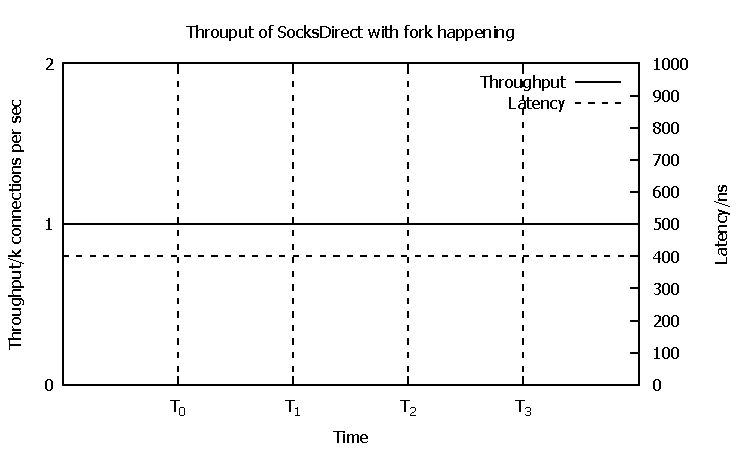
\includegraphics[width=\columnwidth]{eval/microbenchmark/fork-tput.pdf}
%	\caption{Throughput of SocksDirect with fork happening}
%	\label{socksdirect:fig:eval-fork-tput}
%\end{figure}

\sys{} is implemented in three components: a user-space library \libipc{} and a monitoring daemon with 17K lines of C++ code, as well as a kernel module that supports zero-copy.
This section evaluates \sys{} from the following aspects:

\parab {Efficiently using shared memory for intra-host sockets.}
For 8-byte messages, \sys achieves 0.3 $\mu$s RTT and a throughput of 23~M messages per second. For large messages, \sys uses zero-copy to achieve 1/13 of Linux's latency and 26x throughput.

\parab {Efficiently using RDMA for inter-host sockets.}
\sys achieves 1.7 $\mu$s RTT, close to raw RDMA performance.
When zero-copy, a connection can saturate a 100~Gbps link.

%\parab{Robust with number of connections.}
%The performance above can be maintained with up to 100 million connections.

%\parab{Corner-case operations does not affect long-term performance.}
%After corner-case operations such as \texttt{fork}, the performance recovers quickly.

\parab {Scalable with the number of cores.}
As the number of cores increases, the throughput can almost linearly scale.

\parab {Significantly accelerates unmodified end-to-end applications.}
For example, \sys {} reduces the latency of Nginx HTTP requests by 5.5 to 20 times.

\subsection{Evaluation Methodology}
\label{socksdirect:subsec:methodology}

This section evaluates \sys{} on a server with two Xeon E5-2698 v3 CPUs, 256~GiB memory, and a Mellanox ConnectX-4 network card. The server is interconnected with an Arista 7060CX-32S switch via a 100 Gbps Ethernet interface \cite {arista-7060cx}. Unlike Chapters \ref{chapter:clicknp} and \ref{chapter:kvdirect}, this section only uses the commercial card part of the programmable network card, and the commercial card has been upgraded to 100 Gbps, without using FPGA. The server uses Ubuntu 16.04 and Linux 4.15, uses RoCEv2 for the RDMA protocol, and polls the completion queue every 64 messages.
Each thread is pinned to a CPU core. Sufficient warm-up tests were conducted before collecting data.
For latency, this section reports the average round-trip time of a ping-pong application, with error bars representing the 1\% and 99\% percentiles.
For throughput, one side keeps sending data while the other side keeps receiving data.
This section compares Linux, raw RDMA write primitives (write verb), Rsocket~ \cite {rsockets}, and LibVMA~ \cite {libvma}, which is a user-space TCP/IP protocol stack optimized for Mellanox network cards.
We also compared \sys{} without batching and zero-copy, denoted as ``SD (unopt)''.
This section did not evaluate mTCP~ \cite {jeong2014mtcp}, because the underlying DPDK library has limited support for Mellanox ConnectX-4 network cards. Due to batching, mTCP has much higher latency than RDMA, and the reported throughput is 1.7~M packets per second~~ \cite {kalia2018datacenter}.

\subsection{Performance Microbenchmark}
\label{socksdirect:subsec:microbenchmark}

\subsubsection{Latency and Throughput}

Figure \ref {socksdirect:fig:eval-msgsize-intra} shows the intra-host socket performance between a pair of sender and receiver threads.
For 8-byte messages, \sys achieves 0.3 $ \mu $ s round-trip latency (1/35 of Linux) and 23~M messages per second throughput (20 times of Linux).
In comparison, a simple shared memory queue has 0.25 $ \mu $ s round-trip latency and 27~M throughput, indicating that \sys adds very little overhead.
RSocket has 6x latency and 1/4 throughput of \sys  {}, because it uses the network card to forward intra-host packets, which leads to PCIe latency.
LibVMA simply uses kernel TCP sockets for intra-host.
The one-way latency of \sys  {} is 0.15 $ \mu $ s, even lower than kernel crossing (0.2 $ \mu $ s). Kernel-based sockets need to cross the kernel on both the sender and receiver.

Due to memory copying, for 8~KiB messages, the throughput of \sys is only 60% higher than Linux, and the latency is 4 times lower. For messages of at least 16~KiB in size, \sys uses page remapping to achieve zero-copy. For 1~MiB messages, \sys has 1/13 of the latency and 26x the throughput of Linux. Due to event notification latency, the latency of RSocket is unstable and may even be larger than Linux in some cases.

\begin{figure*}[htbp]
	\centering
	\subfloat[Single-machine throughput.]{                    
		\centering
		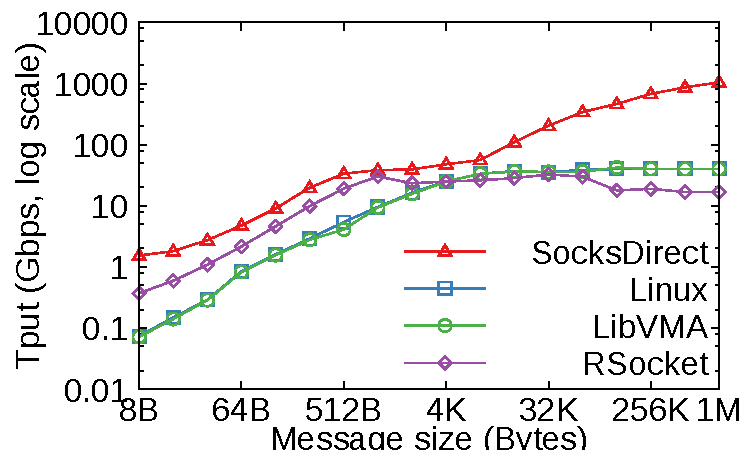
\includegraphics[width=0.5\textwidth]{eval/microbenchmark/msgsize-ipc-tput.pdf}
		\label{socksdirect:fig:eval-msgsize-ipc-tput}
	}
	\subfloat[Single-machine latency.]{
		\centering 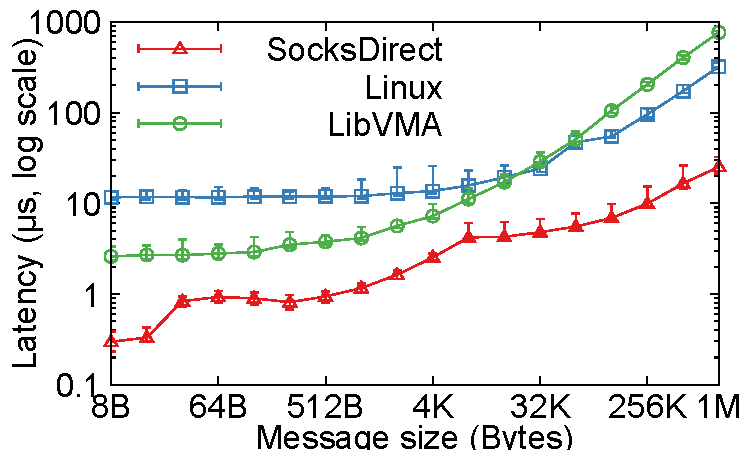
\includegraphics[width=0.5\textwidth]{eval/microbenchmark/msgsize-ipc-lat.pdf}
		\label{socksdirect:fig:eval-msgsize-ipc-lat}
	}
	
	\caption{Single-core message performance of intra-machine communication under different message sizes.}
	\label{socksdirect:fig:eval-msgsize-intra}
\end{figure*}

Figure \ref {socksdirect:fig:eval-msgsize-inter} shows the inter-host socket performance between a pair of threads. For 8-byte messages, \sys{} achieves a throughput of 18M messages per second (15 times that of Linux) and a latency of 1.7 microseconds (1/17 of Linux). The throughput and latency are close to the original RDMA write operation (as shown by the dashed line), which does not have socket semantics. Batching does not affect the latency we evaluate, as RDMA write operations are only delayed when the send queue is full, and we only use one message to evaluate latency. Due to batching, the throughput of \sys  {} for 8-byte messages is even higher than RDMA. The message throughput of non-batching \sys{} is between RSocket and RDMA. LibVMA also uses batching to achieve good performance, but the latency is 7 times that of \sys  {}. For messages smaller than 8~KiB, the throughput of inter-host RDMA is slightly lower than intra-host shared memory because the ring buffer structure is shared. For messages from 512B to 8KiB, and larger messages that do not enable zero-copy, \sys  {} is limited by packet copying, but it is still faster than RSocket and LibVMA due to reduced buffer management overhead. For zero-copy messages ($\ge$ 16 KiB), \sys  {} saturates the network bandwidth, with 3.5 times the throughput of all comparison work and 72% of the latency of RSocket.

\begin{figure*}[htbp]
	\centering
	\subfloat[Cross-host throughput.]{
		\centering 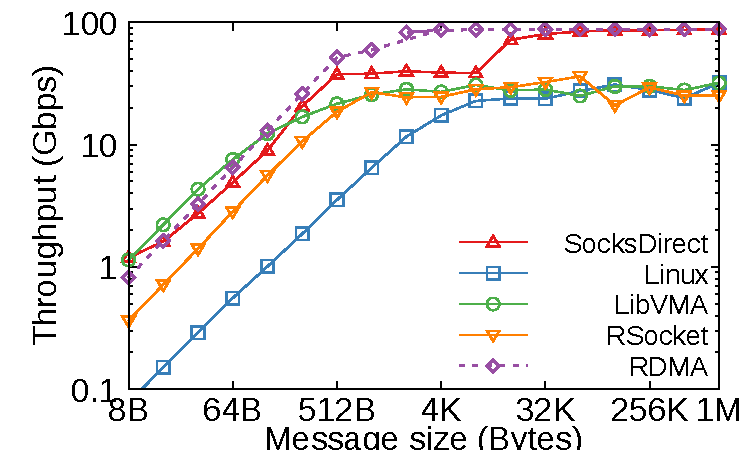
\includegraphics[width=0.5\textwidth]{eval/microbenchmark/msgsize-network-tput.pdf}
		\label{socksdirect:fig:eval-msgsize-network-tput}
	}
	\subfloat[Cross-host latency.]{
		\centering 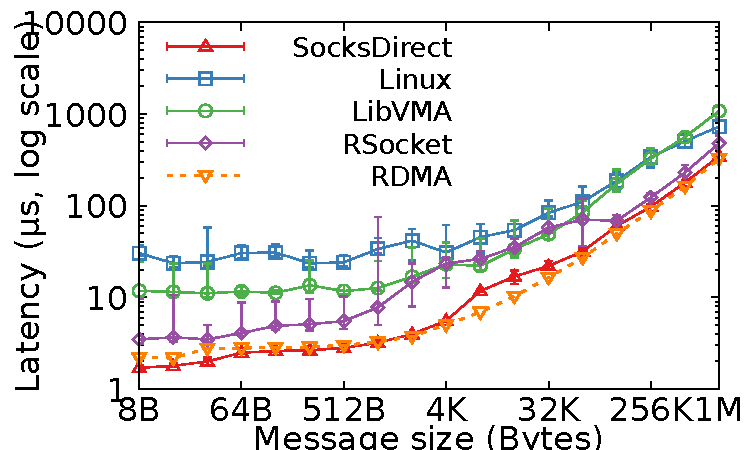
\includegraphics[width=0.5\textwidth]{eval/microbenchmark/msgsize-network-lat.pdf}
		\label{socksdirect:fig:eval-msgsize-network-lat}
	}
	
	\caption{Single-core message performance of cross-host communication under different message sizes.}
	\label{socksdirect:fig:eval-msgsize-inter}
\end{figure*}

\subsubsection{Latency Decomposition}

Table \ref{tab:microbenchmark} explains why the performance of \sys{} surpasses other systems. Each socket operation in Linux requires a kernel traversal, and all systems except \sys{} require locking in thread-safe mode. For each packet, \sys{} saves buffer management overhead and offloads the transport layer and packet processing to the network card. To transmit a packet, \sys{} uses a one-sided RDMA write operation, requiring only one DMA operation at the sender and receiver respectively. RSocket uses two-sided RDMA, and LibVMA uses a similar packet interface, so the receiver needs to add one DMA operation. LibVMA and RSocket use the network card to forward intra-machine packets, while \sys{} uses shared memory. The high latency of Linux is mainly due to interrupt handling and process awakening. For larger messages, \sys{} eliminates data copying, and the overhead of page remapping is significantly lower. RSocket performs better than LibVMA and Linux because it pipelines the data copy operation at the sender, the RDMA send operation, and the data copy operation at the receiver. The connection establishment latency of \sys{} mainly comes from the initial handshake through the Linux raw socket and the creation of RDMA QP through \texttt{libibverbs}.

\begin{table}[htbp]
	\centering
	\small
		\begin{tabular}{l|l|r|r|r|r}
			\hline
			Type & Overhead & \sys & LibVMA & RSocket & Linux \\
			\hline
			\hline
			Per operation & Total (thread-unsafe) & 53 & 56 & 71 & 413 \\
			\hline
			Per operation & Total (thread-safe) & 53 & 177 & 209 & 413 \\
			\hline
			Per operation & C library wrapper & 15 & 10 & 10 & 12 \\
			\hline
			Per operation & Kernel crossing (system call) & N/A & N/A & N/A & 205 \\
			\hline
			Per operation & Socket file descriptor lock & N/A & 121 & 138 & 160 \\
			\hline
			\hline
			Per packet & Total (inter-host) & 850 & 2200 & 1700 & 15000 \\
			\hline
			Per packet & Total (intra-host) & 150 & 1300 & 1000 & 5800 \\
			\hline
			Per packet & Buffer management & 50 & 320 & 370 & 430 \\
			\hline
			Per packet & Transport layer protocol & N/A & 260 & N/A & 360 \\
			\hline
			Per packet & Packet handling & N/A & 200 & N/A & 500 \\
			\hline
			Per packet & NIC doorbell and DMA & 600 & 900 & 900 & 2100 \\
			\hline
			Per packet & NIC handling \& wire & \multicolumn{4}{c}{200} \\
			\hline
			Per packet & Handling NIC interrupt & N/A & N/A & N/A & 4000 \\
			\hline
			Per packet & Process wakeup & N/A & N/A & N/A & 5000 \\
			\hline
			\hline
			Per kilobyte & Total (inter-host)& 173 & 540 & 239 & 365 \\
			\hline
			Per kilobyte & Total (intra-host) & 13 & 381 & 212 & 160 \\
			\hline
			Per kilobyte & Line transmission & \multicolumn{4}{c}{160} \\
			\hline
			\hline
			Per connection & Total (inter-host)& 47000 & 18000 & 77000 & 47000 \\
			\hline
			Per connection & Total (intra-host) & 700 & 3800 & 33000 & 14700 \\
			\hline
			Per connection & Initial TCP handshake & 16000 & 16000 & 47000 & N/A \\
			\hline
			Per connection & Monitor handling & 180 & N/A & N/A & N/A \\
			\hline
			Per connection & RDMA QP creation & 30000 & N/A & 30000 & N/A \\
			\hline
		\end{tabular}
	\caption{Latency breakdown of \sys{} and other systems. The per-operation latency is measured using \texttt{fcntl()}, the per-packet and per-kilobyte latency is the time from \texttt{send()} to \texttt{recv()}, and the per-connection latency is the delay of connection creation. The numbers in the table are in nanoseconds and represent rough estimates.}
	\label{tab:microbenchmark}
\end{table}


\subsubsection{Multi-core Scalability}

\sys has achieved nearly linear scalability for intra-host and inter-host sockets. For intra-host sockets, \sys provides a throughput of 306 M messages per second across 16 pairs of sender and receiver cores, which is 40 times that of Linux and 30 times that of RSocket. LibVMA falls back to Linux for intra-host sockets. Using RDMA as inter-host sockets, \sys achieves a throughput of 276 M messages per second across 16 cores with batching, which is 2.5 times the message throughput of the RDMA network card used in this chapter, and 8 times the throughput of RSocket. Without enabling batching, \sys can only achieve a throughput of 62 M, which is 60% of bare RDMA. Due to the limited scalability of buffer management, the intra-host throughput of RSocket is 24 M, and inter-host is 33 M. Due to lock contention on the shared network card queue, the throughput of LibVMA decreases to 1/4 with two threads compared to single-threaded, and 1/10 with three or more threads. Linux throughput scales linearly from 1 to 7 cores and bottlenecks on loopback or network card queues with more cores. Although not tested in this paper, mTCP is expected to have better scalability in multi-core scenarios.

\begin{figure*}[htbp]
	\subfloat[Single machine throughput.]{                    
		%\begin{minipage}{0.4\textwidth}
		\centering
		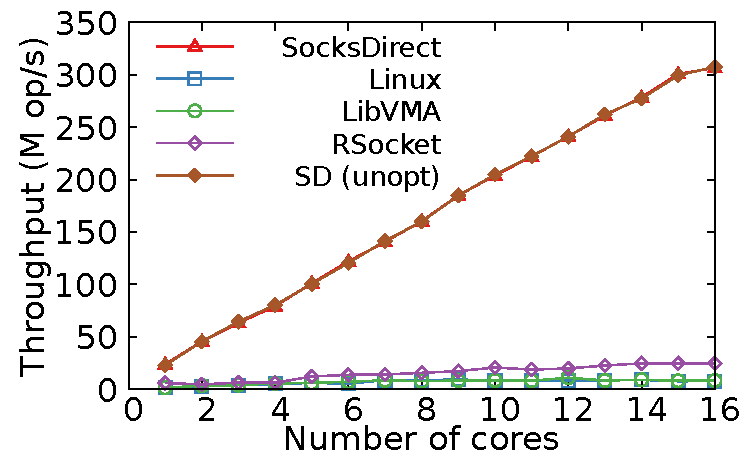
\includegraphics[width=0.5\textwidth]{eval/microbenchmark/corenum-IPC-tput.pdf}
		\label{socksdirect:fig:eval-cornum-ipc}
		%\end{minipage}
	}
	\subfloat[Cross-host throughput.]{
		%\begin{minipage}{0.4\textwidth}
		\centering 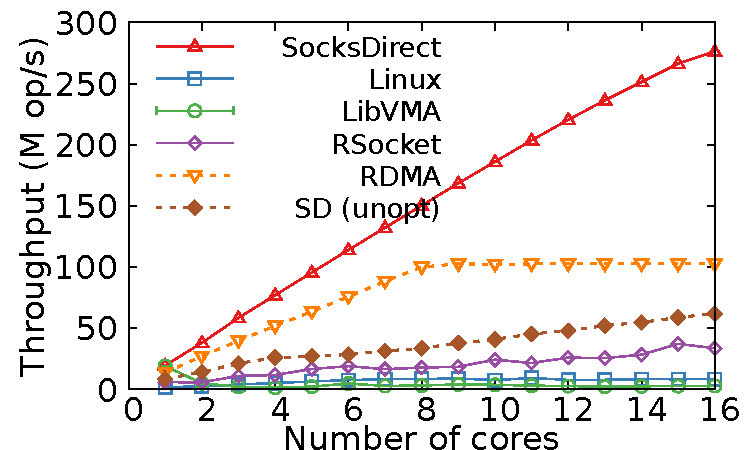
\includegraphics[width=0.5\textwidth]{eval/microbenchmark/corenum-network-tput.pdf}
		\label{socksdirect:fig:eval-cornum-network}
		%\end{minipage}
	}
	
	\caption{Throughput of 8-byte messages under different CPU core numbers.}
	\label{socksdirect:fig:eval-corenum-tput}
\end{figure*}


%The multi-thread scalability of \sys  attributes to the partitioning of states and removal of synchronization.
%We can also see that shared memory communication has 5x throughput than RDMA.% Using RDMA 网卡 for intra-host socket would meet this bottleneck and thus not scalable.

%Figure~\ref{socksdirect:fig:eval-conn-setup-tput} shows the throughput of connection creation with different number of cores. Each core can create 1.4~M new connections per second, which is 20x of Linux and 2x of mTCP~\cite{jeong2014mtcp}. The upper bound is 5.3~M connections per second, where the monitor becomes a bottleneck.

Finally, we evaluate the performance of multiple threads sharing a core. Each thread has to wait for its turn to process messages.
As shown in Figure \ref {socksdirect:fig:eval-context-switch}, although the message processing latency almost linearly increases with the number of active processes, it is still 1/20 to 1/30 of that of Linux.


\begin{figure}[htbp]
	%\centering
	%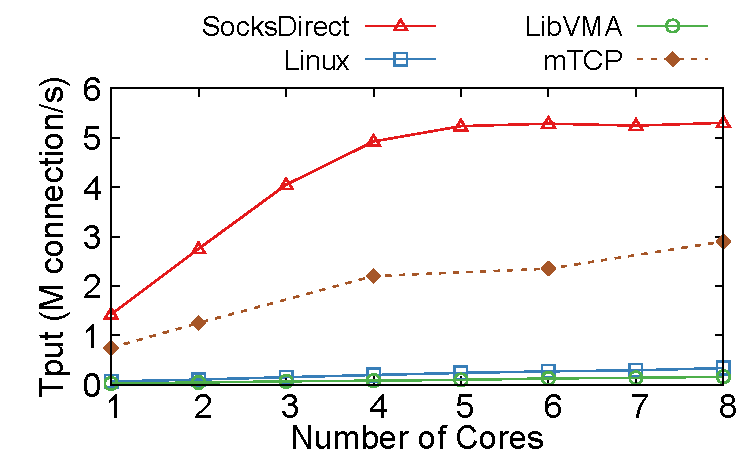
\includegraphics[width=\textwidth]{eval/microbenchmark/conn-setup-tput.pdf}
	%
	%\caption{Connection creation throughput with number of cores.}
	%\label{socksdirect:fig:eval-conn-setup-tput}
	
	%\begin{minipage}{0.4\textwidth}
	\centering 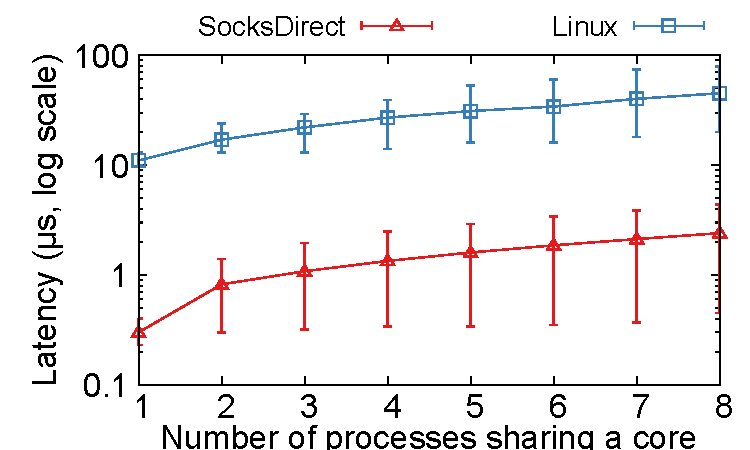
\includegraphics[width=0.5\textwidth]{eval/microbenchmark/sharecore-lat.pdf}
	
	\caption{Message processing latency when multiple processes share a CPU core.}
	\label{socksdirect:fig:eval-context-switch}
	%\end{minipage}
\end{figure}


%Finally, we benchmark the throughput and latency after \texttt{fork} and other corner-case operations. Initially, there is only one pair of sender and receiver. At time $T_0$, receiver forks, and the parent process keeps receiving. At time $T_1$, the child process begins to receives takes over the socket. At time $T_2$, sender forks, and only the parent sends. At time $T_3$, the child sender also starts sending. We find that both throughput and latency resume to initial maximal performance within 1~ms after each event.

